% !TEX root = ../integrado.tex
En la figura \ref{fig:infoInscripciones} se muestra el modelado de los datos que serán utilizados en el \refElem{Calmecac} para el proceso de inscripciones.

\begin{figure}[hbtp!]
	\begin{center}
	\fbox{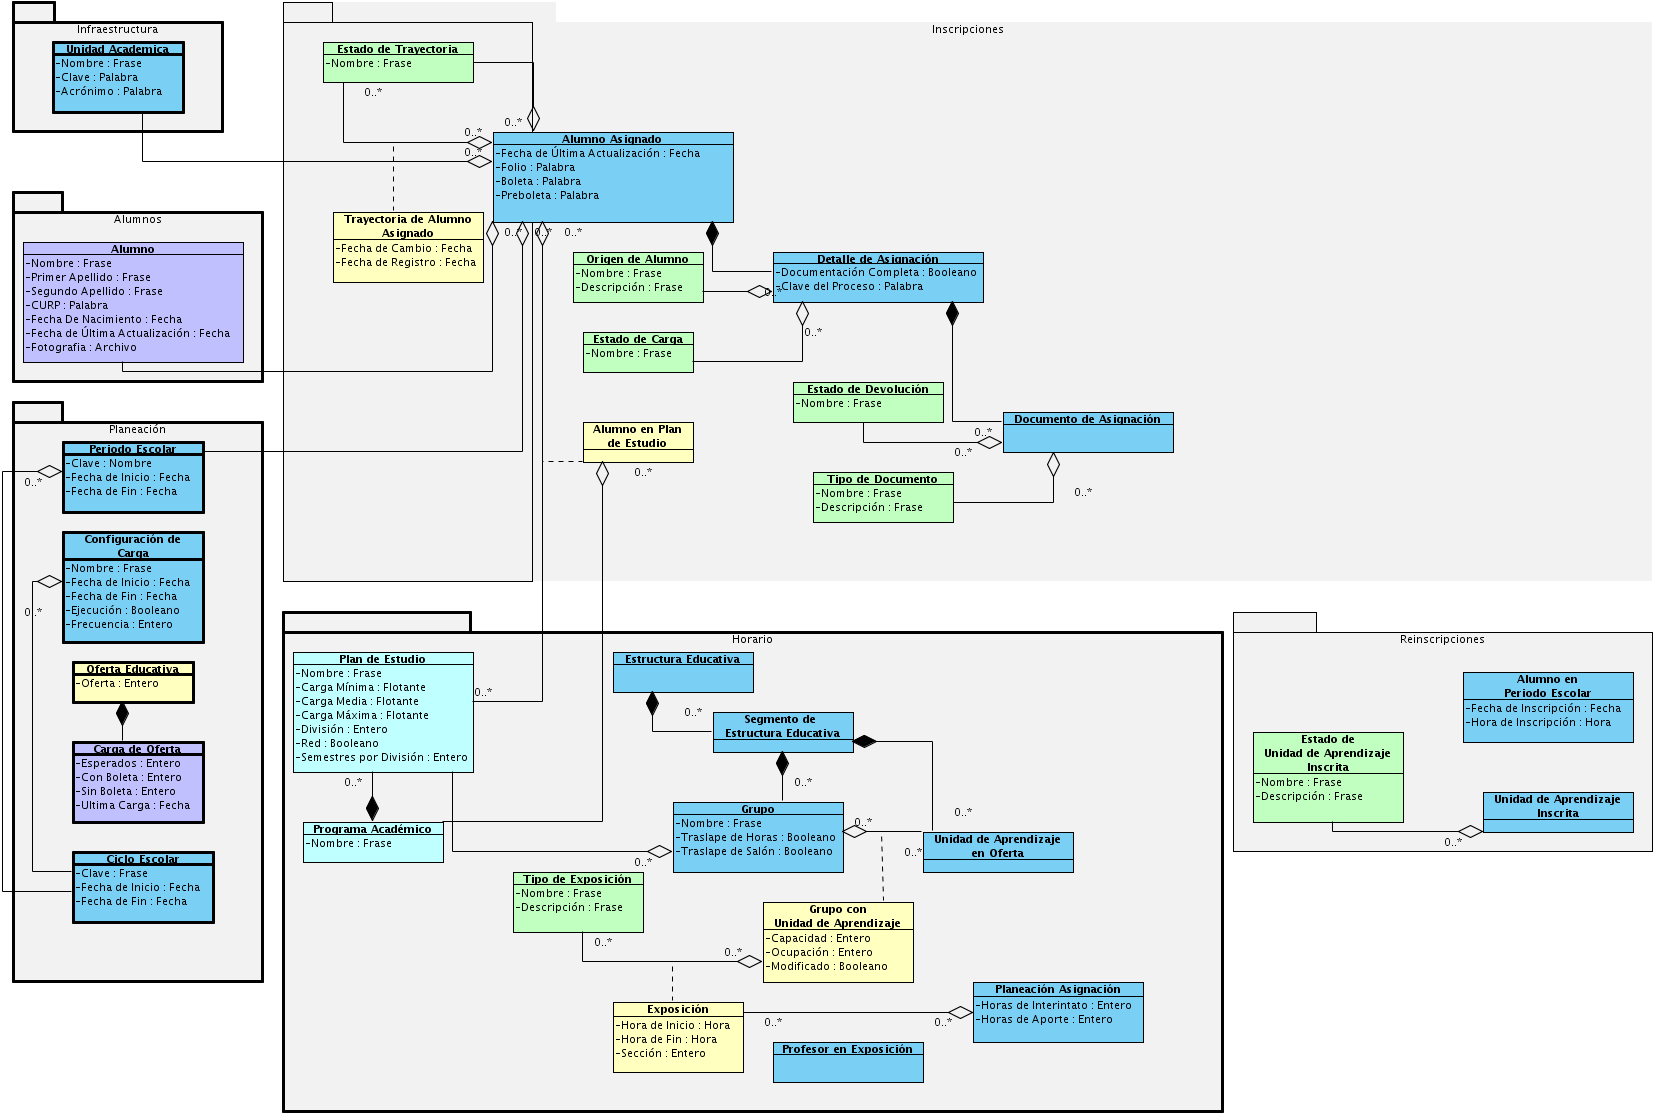
\includegraphics[width=\textwidth]{negocio/images/Inscripciones_MDI}}
		\caption{Modelo de Información de Inscripciones}
		\label{fig:infoInscripciones}
	\end{center}
\end{figure}

\section{Planeación}

	Cada cierto periodo de tiempo en el Instituto se forma una comisión en la que se delibera y establecen los eventos académicos con más relevancia para la comunidad, dando como resultado la estructuración y conformación del Calendario Académico por medio del cual una o varios Unidades Académicas se regirán para la realización de actividades. En este calendario se establecen los periodos de evaluación, los periodos para reinscripciones e inscripciones, los periodos para la aplicación de E.T.S. así como las fechas feriadas.\\

% CICLO ESCOLAR
\begin{cdtEntidad}[Lapso anual que define el Calendario Académico del Instituto Politécnico Nacional.]{CicloEscolar}{Ciclo Escolar}%REGLAMENTO General de Estudios pagina 7
		\brAttr{clave}{Clave}{palabra}{Es el conjunto de caracteres que denotan a un lapso anual en el cual se llevan a cabo actividades administrativas y de docencia.}{\datRequerido}%check
		
	\brAttr{fechaDeInicio}{Fecha de Inicio}{fecha}{Específica el día en el año en que el ciclo escolar da inicio y que sirve como base para la definición del comienzo de sus calendarios académicos. Este dato es relativo a cada Unidad Académica o Calendario Académico.}{\datOpcional}
	
	\brAttr{fechaDeTermino}{Fecha de Término}{fecha}{Específica el día en el año en que el ciclo escolar concluye y que sirve como base para la definición del término de sus calendarios académicos. Este dato es relativo a cada Unidad Académica o Calendario Académico.}{\datOpcional}
	
	\cdtEntityRelSection
	
	\brRel{\brRelComposition}{\refElem{CalendarioAcademico}}{En un Ciclo Escolar se {\bf elaboran} uno o más Calendarios Académicos para coordinar y supervisar las actividades de gestión escolar.}% Reglamento orgánico pag. 34
	
	\brRel{\brRelComposition}{\refElem{PeriodoEscolar}}{En un Ciclo Escolar {\bf se señalan}  dos Periodos Escolares para cursar unidades de aprendizaje.} % Reglamento general de estudios, pag. 8
	
	% TODO: Referenciar a la entidad
	% TODO: ?`Se debe quitar?
	\brRel{\brRelAgregation}{\refElem{UnidadAcademica}}{Una Unidad Académica {\bf opera} durante uno o más Ciclo Escolar y esto es de acuerdo a los programas académicos que ofrece y sus modalidades.}% 

\end{cdtEntidad}

% CALENDARIO ACADÉMICO
\begin{cdtEntidad}[Es la planeación y estructuración que define los tiempos en programación que define se realizan anualmente las actividades académicas y de gestión escolar, en las diversas modalidades educativas que imparte el Instituto.]{CalendarioAcademico}{Calendario Académico}% Reglamento general de estudios pag. 7

	\brAttr{nombre}{Nombre}{frase}{Es la palabra o el conjunto de palabras que denotan e identifican la definición de tiempos para realizar las actividades académicas y de gestión escolar en una o varias Unidades Académicas y para modalidades distintas. }{\datRequerido}

	\cdtEntityRelSection
	
	\brRel{\brRelComposition}{\refElem{CicloEscolar}}{A un Ciclo Escolar se le definen los Calendarios Académicos que sirven para estructurar y conformar los periodos de tiempo en que se llevan a cabo actividades académicas y de gestión.}

	\brRel{\brRelComposition}{\refElem{ActividadCalendario}}{Un Calendario Académico esta {\bf constituido} por un conjunto de tareas académicas y de gestión definidas para llevarse a cabo en un periodo de tiempo el cual debe estar dentro de los limites de un ciclo escolar. }

	% TODO: Referenciar a la entidad
	\brRel{\brRelAgregation}{\refElem{UnidadAcademica}}{Un Calendario Académico {\bf aplica} para un conjunto de Unidades Académicas, las cuales llevarán a cabo sus actividades administrativas y  académicas con base en la planeación definida en el Calendario.}

%	Se eliminará porque es un catálogo
%	\brRel{\brRelAgregation}{\refElem{Modadlidad}}{Una unidad académica se rige por uno o varios calendarios  dependiendo de sus programas académicos y sus modalidades.}
	
	\brRel{\brRelAgregation}{\refElem{CalendarioAcademico}}{Un Calendario Académico puede tener un {\bf Calendario Hijo}, cuando este requiere ser especificado para una Unidad Académica. Y un Calendario Académico puede tener un {\bf Calendario Base} si y solo si ha sido especificado para una Unidad Académcia.}
	
\end{cdtEntidad}

% PERIODO ESCOLAR
\begin{cdtEntidad}[Es el lapso señalado en el Calendario Académico para cursar Unidades de Aprendizaje de un Programa Académico.]{PeriodoEscolar}{Periodo Escolar}% Reglamento general de estudios pag. 8

	\brAttr{clave}{Clave}{frase}{Es el conjunto de caracteres que identifica el lapso de tiempo dentro de un ciclo escolar en el que se cursan Unidades de Aprendizaje definidas por la estructura educativa determinada en un periodo escolar.}{\datRequerido}
	
	\brAttr{fechaInicio}{Fecha de Inicio}{fecha}{Indica el día en el que inicia el lapso de tiempo para cursar Unidades de Aprendizaje de un Programa Académico.}{\datRequerido}
	
	\brAttr{fechaTermino}{Fecha de Término}{fecha}{Indica el día en el que concluye el lapso de tiempo para cursar Unidades de Aprendizaje de un Programa Académico.}{\datRequerido}
	
	\cdtEntityRelSection
	
	\brRel{\brRelComposition}{\refElem{CicloEscolar}}{Un Periodo Escolar es {\bf señalado} dentro de un Ciclo Escola.}

	\brRel{\brRelComposition}{\refElem{ActividadCalendario}}{En un Periodo Escolar {\bf se definen}  las actividades que determinan las acciones que cada Unidad Académica que conforman el Calendario Académico.}

	% Rev. Ulises Vélez: Ok. 
	\brRel{\brRelAgregation}{\refElem{UnidadAcademica}}{En un Periodo Escolar se {\bf ofertan} Programas Académicos por las Unidades Académicas.}
		
\end{cdtEntidad}

%ACTIVIDAD CALENDARIO
\begin{cdtEntidad}[Es una lapso de tiempo en el que una actividad académica debería realizarse.]{ActividadCalendario}{Actividad de Calendario}
	
	\brAttr{fechaInicio}{Fecha de Inicio}{fecha}{Es el día dentro de un Ciclo Escolar en el que se define el comienzo de una Actividad que pertenece al Calendario Académico y que las Unidades Académicas asociadas a ese Calendario deberán comenzar a realizar.}{\datRequerido}
	
	\brAttr{fechaFin}{Fecha de Fin}{fecha}{Es el día dentro de un Ciclo Escolar en el que se define el la conclusión de una Actividad que pertenece al Calendario Académico y que las Unidades Académicas asociadas a ese Calendario deberán finalizar.}{\datRequerido}

	\cdtEntityRelSection
		
	\brRel{\brRelComposition}{\refElem{PeriodoEscolar}}{Una Actividad de Calendario se {\bf realiza} dentro de un Periodo Escolar.}

\end{cdtEntidad}

% CICLO DE UNIDAD ACADÉMICA
\begin{cdtEntidad}[\TODO]{TipoDeActividad}{Tipo de Actividad}
\end{cdtEntidad}

% CALENDARIO DE UNIDAD
\begin{cdtEntidad}[\TODO]{Actividad}{Actividad}
\end{cdtEntidad}

%-------------------------------------Configuración de Proceso de Inscripción--------------------------------------
\section{Configuración de Proceso de Inscripción}

Es el proceso de la importación de los aspirantes de nuevo ingreso, de cambio de carrera o alumno de movilidad cuya información será actualizada e importada al CALMÉCAC.

% PROGRAMA 
\begin{cdtEntidad}[Es la programación del proceso de importación de aspirantes y actualización de información desde el sistema de Admisión.]{Programa}{Programa}

	\brAttr{nombre}{Nombre}{frase}{Identificador de la programación del proceso.}{\datRequerido}

	\brAttr{estado}{Estado}{entero}{Indica el estado en el que se encuentra el proceso: En ejecución o detenido.}{\datRequerido}

	\brAttr{fechaInicio}{Fecha de Inicio}{fecha}{Indica la fecha y hora en la que el proceso debe empezar a ejecutarse periódicamente de acuerdo a la Frecuencia de Ejecución.}{\datRequerido}
	
	\brAttr{fechaTermino}{Fecha de Término}{fecha}{Indica la fecha y hora en la que el proceso debe dejar de ejecutarse periódicamente.}{\datRequerido}
	
	\brAttr{confirmacionAutomatica}{Confirmación Automática}{boleano}{Indica el valor del atributo ``confirmado'' que debe tener por defecto un Aspirante al ser importad. Por defecto es ``verdadero''. No se usa.}{\datRequerido}
	
	\brAttr{frecuenciaDeEjecucion}{Frecuencia de Ejecución}{entero}{Indica la frecuencia con que debe ejecutarse el proceso, indicando la cantidad como un valor entero y la unidad de medida de esta cantidad corresponde a la ``Parte Fecha''.}{\datRequerido}
	
	\cdtEntityRelSection
	
	\brRel{\brRelComposition}{\refElem{Parte Fecha}}{Un Programa se {\bf ejecuta} cada cierto tiempo (indicado en Frecuencia de Ejecución) expresado en {\bf Parte Fecha}.}
	\brRel{\brRelComposition}{\refElem{Corrida}}{La ejecución de un Programa {\bf se registra en} una Corrida.}

\end{cdtEntidad}

% CORRIDA
\begin{cdtEntidad}[Es el registro de la ejecución del proceso de inscripción]{Corrida}{Corrida}

	\brAttr{duracion}{Duración}{hora}{Indica el tiempo medido en milisegundos transcurrido durante la ejecución del proceso.}{\datRequerido}
	
	\brAttr{fechaDeEjecucion}{Fecha de Ejecución}{fecha}{Día y hora en el que el proceso de inscripción inició su ejecución.}{\datRequerido}
	
	\brAttr{resultado}{Resultado}{frase}{Texto que indica el resultado de la ejecución. Debe indicar que la ejecución fue correcta o describir textualmente las fallas que se encontraron durante la ejecución.}{\datRequerido}
	
	\cdtEntityRelSection
	
	\brRel{\brRelComposition}{\refElem{Programa}}{Una Corrida {\bf registra} la ejecución de un Programa.}
	
\end{cdtEntidad}

%-------------------------------------Infraestructura--------------------------------------
\section{Infraestructura}

\TODO

% Unidad Académica
\begin{cdtEntidad}[\TODO]{UnidadAcademica}{Unidad Académica}

	\brAttr{nombre}{Nombre}{frase}{Es la palabra o el conjunto de palabras que denotan e identifican a la Unidad Académica.}{\datRequerido}

	\brAttr{clave}{Clave}{frase}{Es el conjunto de caracteres que identifica a la Unidad Académica en el Instituto.}{\datRequerido}

	\brAttr{acronimo}{Acrónimo}{palabra}{Palabra formada por las iniciales de la Unidad Académica que la identifican en el Instituto.}{\datRequerido}
		
	\cdtEntityRelSection
	
	\brRel{\brRelAgregation}{\refElem{PeriodoEscolar}}{\TODO}
	
	\brRel{\brRelAgregation}{\refElem{CicloEscolar}}{\TODO}
	
	\brRel{\brRelAgregation}{\refElem{CalendarioAcademico}}{\TODO}
	
\end{cdtEntidad}

%%%%%%%%%%%%%%%%%%%%%Horarios
\section{Horarios}

Una Unidad Académica realiza semestralmente la planeación relacionada a la distribución de Unidades de Aprendizaje en espacios y horarios, así como de asignación de Profesores que realizaran las exposiciones para el periodo definido por la Estructura Educativa. En el caso de los profesores cuya relación con el Instituto se define por un contrato se requerirá la justificación que soporte la falta de horas frente a grupo. A toda esta planeación se le conoce como Estructura Educativa y es uno de los procesos más grandes y complejos del Instituto, ya que requiere de la más alta cooperación entre las distintas áreas internas y externas de una Unidad Académica.\\

En el paquete de \textit{Horarios} se verán reflejadas las relaciones entre las entidades que permiten ejecutar está operación y cómo se almacenarán en el sistema para su consulta y edición.\\

\begin{cdtEntidad}[Es la entidad que integra todos los planes de estudios ofertados por las Unidades Académicas del Instituto.]{PlanDeEstudio}{Plan de Estudio}

	\brAttr{cargaMinima}{Carga Mínima de Créditos}{flotante}{Es un dígito que representa el cálculo obtenido de dividir el número total de créditos del programa académico entre el número de periodos escolares de la duración máxima del plan de estudio.}{\datOpcional}
	
	\brAttr{cargaMedia}{Carga Media de Créditos}{flotante}{Es un dígito que representa el cálculo obtenido de al dividir el número total de créditos del programa académico entre el número de periodos escolares de la duración máxima del plan de estudio}{\datOpcional}
	
	\brAttr{cargaMaxima}{Carga Máxima de Créditos}{flotante}{Es un dígito que representa el cálculo obtenido de dividir  el número total de créditos del programa académico entre el número de periodos escolares de la duración mínima del plan de estudio.}{\datOpcional}
	
	\brAttr{division}{División}{entero}{Es un dígito que representa el número segmentaciones que un Plan de Estudios tiene para ubicar sus Unidades de Aprendizaje.}{\datRequerido}
	
	\brAttr{red}{Red}{entero}{Indica si el Plan de Estudio es compartido e impartido entre distintas Unidades Académicas.}{\datOpcional}
	
	\brAttr{planDeEstudio}{Plan de Estudio}{frase}{Es la palabra o conjunto de palabras que representan e identifica a la estructura curricular derivada de un Programa Académico.}{\datOpcional}
	
	
	\cdtEntityRelSection
	
	\brRel{\brRelAgregation}{\refElem{PeriodoEnUnidadAcademica}}{El plan de estudio de un programa académico es ofertado en una unidad académica durante uno o más periodos escolares.}
	
\end{cdtEntidad}

\section{Inscripciones}

\begin{cdtEntidad}[Son los Programas Académicos que oferta cada Unidad Académica en Cada Periodo Escolar.]{PeriodoEnUnidadAcademica}{Periodo en Unidad Académica}

	\brAttr{fechaInicio}{Fecha de Inicio}{fecha}{Indica el día en que inicia la oferta de un démico en un Periodo Escolar y Unidad Académica.}{\datRequerido}
	
	\brAttr{fechaTermino}{Fecha de Término}{fecha}{Indica el día en que concluye la oferta de un Programa Académico en un Periodo Escolar y Unidad Académica.}{\datRequerido}
	
	\cdtEntityRelSection
	
	\brRel{\brRelComposition}{\refElem{PlanDeEstudio}}{Un Periodo en Unidad Académica {\em especifica una oferta} de un Plan de Estudios.}
	\brRel{\brRelComposition}{\refElem{UnidadAcademica}}{Un Periodo en Unidad Académica {\em especifica una oferta} en una Unidad Académica}
	\brRel{\brRelComposition}{\refElem{PeriodoEscolar}}{Un Periodo en Unidad Académica {\em especifica una oferta} en un Periodo Escolar.}
\end{cdtEntidad}


%\TODO: En el MDI cambiar Plan de Estudios por Plan de Estudio
\begin{cdtEntidad}[Agrupa y los ingresos de Aspirantes a Planes de Estudios de Unidades Académicas por Tipo de Carga]{PlanDeEstudioEnPeriodoDeUnidadAcademica}{Plan de Estudio en Periodo de Unidad Académica}
	
	\brAttr{oferta}{Oferta}{entero}{Es el número de estudiantes esperados (lugares disponibles) para inscribir Alumnos de nuevo ingreso a un Plan de Estudio Ofertado en un Periodo Escolar.}{\datRequerido}
	
	\brAttr{estudiantesEsperados}{Estudiantes Esperados}{entero}{Es el número de estudiantes esperados (lugares disponibles) para inscribir Alumnos de nuevo ingreso a un Plan de Estudio Ofertado en un Periodo Escolar.}{\datRequerido}
	
	\brAttr{estudiantesCargadosConBoleta}{Estudiantes Cargados con Boleta}{entero}{Es el número de alumnos de nuevo ingreso que {\bf cuentan} con número de Boleta para el Plan de Estudios, Unidad Académica y Periodo Escolar correspondiente y que {\bf no han sido inscritos}.}{\datRequerido}
	
	\brAttr{estudiantesCargadosSinBoleta}{Estudiantes Cargados sin Boleta}{entero}{Es el número de alumnos de nuevo ingreso que {\bf no cuentan} con número de Boleta para el Plan de Estudios, Unidad Académica y Periodo Escolar correspondiente y que {\bf no han sido inscritos}.}{\datRequerido}
	
	\brAttr{estudiantesInscritosSinBoleta}{Estudiantes Inscritos sin Boleta}{entero}{Es el número de alumnos de nuevo ingreso que {\bf no cuentan} con número de Boleta para el Plan de Estudios, Unidad Académica y Periodo Escolar correspondiente y que {\bf ya han sido inscritos}.}{\datRequerido}
	
	\brAttr{estudiantesInscritosConBoleta}{Estudiantes Inscritos con Boleta}{entero}{Es el número de alumnos de nuevo ingreso que {\bf cuentan} con número de Boleta para el Plan de Estudios, Unidad Académica y Periodo Escolar correspondiente y que {\bf ya han sido inscritos}.}{\datRequerido}
	
	\brAttr{estudiantesCancelados}{Estudiantes Cancelados}{entero}{Es el número de alumnos de nuevo ingreso cuyo ingreso al IPN se encuentra en proces de cancelación por los motivos establecidos en el \textbf{Artículo 14} del \textbf{Reglamento General de Estudios}.}{\datRequerido}
	
	\brAttr{fechaDeUltimaActualizacion}{Fecha de Última Actualización}{fecha}{Indica el día y la hora en que esta información ha sido modificada por última vez.}{\datOpcional}
	% TODO: Debería ser ``Convocatoria''.
	\brAttr{tipoDeCarga}{Tipo de Carga}{TipoDeCarga}{Indica el tipo de carga realizado.}{\datRequerido}
	
	\cdtEntityRelSection
	
	\brRel{\brRelComposition}{\refElem{AlumnoAsignado}}{A un Plan de Estudio en Periodo de Unidad Académica {\bf se le asignan} Alumnos Asignados.}
	
\end{cdtEntidad}


\begin{cdtEntidad}[Es un aspirante o alumno que al haber aprobado el examen de Admisión y que cumple con los requisitos de la convocatoria correspondiente es asignado a un plan de estudio ofertado por una Unidad Académica en un periodo escolar. Tiene como propósito especificar si el aspirante tiene la documentación requerida para completar el proceso de Inscripción o si requiere realizar una corrección o si su asignación debe ser anulada.]{AlumnoAsignado}{Alumno Asignado}

	\brAttr{observacionesDeDocumentacion}{Observaciones de Documentación}{texto}{Especifica las observaciones del personal de Gestión Escolar en caso de que no haya sido satisfactoria la entrega de documentos a un Aspirante una vez que haya completado su Inscripción y se le haya asignado su número de Boleta.}{\datOpcional}
	
	\brAttr{folio}{Folio}{palabra}{Identificador del aspirante junto con Clave en el proceso, utilizado únicamente durante el proceso de admisión.}{\datRequerido}
	
	\brAttr{claveEnElProceso}{Clave del Proceso}{palabra}{Indica el proceso mediante el cual el aspirante fue asignado: Convocatoria de nuevo ingreso, movilidad, cambio de carrera, RVOE, etc.}{\datRequerido}
	
	\brAttr{preboleta}{Preboleta}{palabra}{Identificador del estudiante mientras no cuente con Boleta. Permite identificar el tipo u origen del alumno.}{\datOpcional}
	
	\brAttr{boleta}{Boleta}{palabra}{Identificador del Alumno dentro del Instituto. Su asignación le permite tener todos los derechos como estudiante. Al no contar con Boleta al estudiante se le denomina Aspirante.}{\datOpcional}
	
	\brAttr{fechaDeUltimaCarga}{Fecha de Última Carga}{fecha}{Indica fecha y hora de la última  actualización la información.}{\datOpcional}
	
	\brAttr{estadoDeCargaDelAlumno}{Estado de Carga del Alumno}{EstadoDeCargaDelAlumno}{Indica la condición en la que se encuentra un Aspirante después de que se realiza una carga en el sistema de la información de su documentación o de su asignación de boleta o preboleta.}{\datRequerido}
	
	\brAttr{estadoDeDocumentacion}{Estado de Documentación}{EstadoDeDocumentacion}{Indica si a un Alumno Asignado con Boleta se le ha entregado la documentación o si dicha entrega tiene observaciones.}{\datRequerido}
		
	\brAttr{estadoDelAlumno}{Estado del Alumno}{EstadoDelAlumno}{Indica el estado en el que se encuentra el Alumno.}{\datRequerido}
	
	\cdtEntityRelSection
	
	\brRel{\brRelAgregation}{\refElem{Documento}}{A un Alumno Asignado se le {\bf entregan} Documentos.}
	
	\brRel{\brRelComposition}{\refElem{SituacionEscolar}}{Un Alumno Asignado {\bf tiene} una Situación Escolar.}
	
	\brRel{\brRelComposition}{\refElem{Alumno}}{Un Alumno Asignado {\bf es} un Alumno.}


\end{cdtEntidad}


\begin{cdtEntidad}[\TOCHK Es la condición que un Alumno Asignado tiene en un Plan de Estudios. Indica algunas propiedades que permiten efectuar operaciones en el sistema de parte del Alumno así como de otros procesos que lo involucren.]{SituacionEscolar}{Situación Escolar}

	\brAttr{promedioGeneral}{Promedio General}{flotante}{Es el número que indica resultado de efectuar la suma de las calificaciones obtenidas de las Unidades de Aprendizaje Cursadas entre el número de Unidades de Aprendizaje Cursadas.}{\datOpcional}
	
	\brAttr{creditosObtenidos}{Créditos Obtenidos}{flotante}{Es el número que indica el resultado de efectuar la suma de los créditos S.A.T.C.A. de las Unidades de Aprendizaje Cursadas y cuya calificación es mayor a la mínima aprobatoria de acuerdo al \textbf{Artículo 40} del \textbf{Reglamento General de Estudios}. Tiene como propósito ser uno de los mecanismos que indiquen el grado de avance del Alumno en el plan de estudio.}{\datOpcional}
	
	\brAttr{creditosFaltantes}{Créditos Faltantes}{flotante}{Es el número que indica el resultado de efectuar la resta de los créditos totales de un plan de estudios con los obtenidos por el Alumno. Tiene como propósito ser uno de los mecanismos que indiquen el grado de avance del Alumno en el plan de estudio. }{\datOpcional}
	
	\brAttr{uDeAAprobadas}{Unidades de Aprendizaje Aprobadas}{entero}{Es el número que indica la cantidad de Unidades de Aprendizaje de un plan de estudio que un Alumno ha acreditado.}{\datOpcional}
	
	\brAttr{uDeAReprobadas}{Unidades de Aprendizaje Reprobadas}{entero}{Es el número que indica la cantidad de Unidades de Aprendizaje de un plan de estudio que no ha acreditado.}{\datOpcional}
	
	\brAttr{uDeADesfasadas}{Unidades de Aprendizaje Desfasadas}{entero}{Es el número que indica las unidades de aprendizaje que entran en el siguiente criterio: ´´\textit{Ningún alumno podrá cursar asignaturas o equivalentes que correspondan a más de tres periodos escolares consecutivos y no podrá adeudar las correspondientes de más de dos periodos escolares previos al que curse.}''}{\datOpcional}
	
	\brAttr{semestreActual}{Semestre Actual}{entero}{\TOCHK Es el número que indica el semestre en el que se encuentra un Alumno con base en el plan de estudio y las Unidades de Aprendizaje inscritas en el periodo corriente. }{\datOpcional}
	
	\brAttr{periodosTranscurridos}{Periodos Transcurridos}{entero}{\TOCHK Es el número que indica la cantidad de periodos en los que un alumno ha inscrito Unidades de Aprendizaje.}{\datOpcional}
	
	\brAttr{periodosDeBajaTemporal}{Periodos de Baja Temporal}{entero}{\TOCHK Es el número que indica la cantidad de periodos en los que un Alumno no ha efectuado una reinscripción pero cuya justificación se encuentra apoyada por un documento aprobado por el Director de la Unidad Académica a la cual el Alumno fue asignado.}{\datOpcional}
	
	\brAttr{porcentajeDeCreditos}{Porcentaje de Créditos}{flotante}{\TOCHK Es un número que representa el resultado de efectuar la suma de los créditos S.A.T.C.A. obtenidos entre el total de las Unidades de Aprendizaje del plan de estudio. }{\datOpcional}
	
	\brAttr{periodosEstimados}{Periodos Estimados}{entero}{\TODO}{\datOpcional}
	
\end{cdtEntidad}


\begin{cdtEntidad}[Es el resultado de la relación de \refElem{tdDocumento} y \refElem{AlumnoAsignado} y tiene como propósito almacenar todos los documentos que son requeridos para el proceso de Inscripción del Instituto y que fueron entregados por el Aspirante.]{DocumentoDeAlumnoAsignado}{Documento de Alumno Asignado}

	\brAttr{estadoDevolucionDocumento}{Estado de Devolución de Documento}{EstadoDeDevolucionDeDocumento}{Indica la condición que presenta un documento entregado por un Aspirante y tiene como propósito definir si el documento ha sido entregado de forma satisfactoria o si requiere de una corrección.}{\datRequerido}

\end{cdtEntidad}